\chapter{IBM BigFix}

\section{BigFix}
I prodotti della suite IBM BigFix consentono di monitorare e gestire in tempo reale un elevato numero di dispositivi fisici e virtuali connessi (fino a 250.000). Questi possono essere sia fisici che virtuali, come ad esempio server, desktop, notebook, dispositivi mobili, tablet, POS, ATM, chioschi self-service. Gli utenti principali di questi prodotti sono gli amministratori di sistema. Tramite le applicazioni BigFix possono avere il pieno controllo sugli endpoint, come distribuire software, applicare delle patch, effettuare il deploy di sistemi operativi, proteggere da attacchi di rete e molto altro.
\subsection{Architettura}
Un'architettura di BigFix è, per sua natura, molto articolata, poichè la necessità e quella di gestire un numero elevato ed eterogeneo di dispositivi. Essa si basa sul consolidato pattern stilistico Client/Server, ma con una struttura leggermente variata, prevedendo l'inserimento di un ulteriore layer frapposto tra client e server, i relay, i quali sono fondamentali per bilanciare il carico.
\paragraph{}
Ma partiamo subito con un esempio per avere un ponto di riferimento.
\begin{figure}[h!]
	\centering
	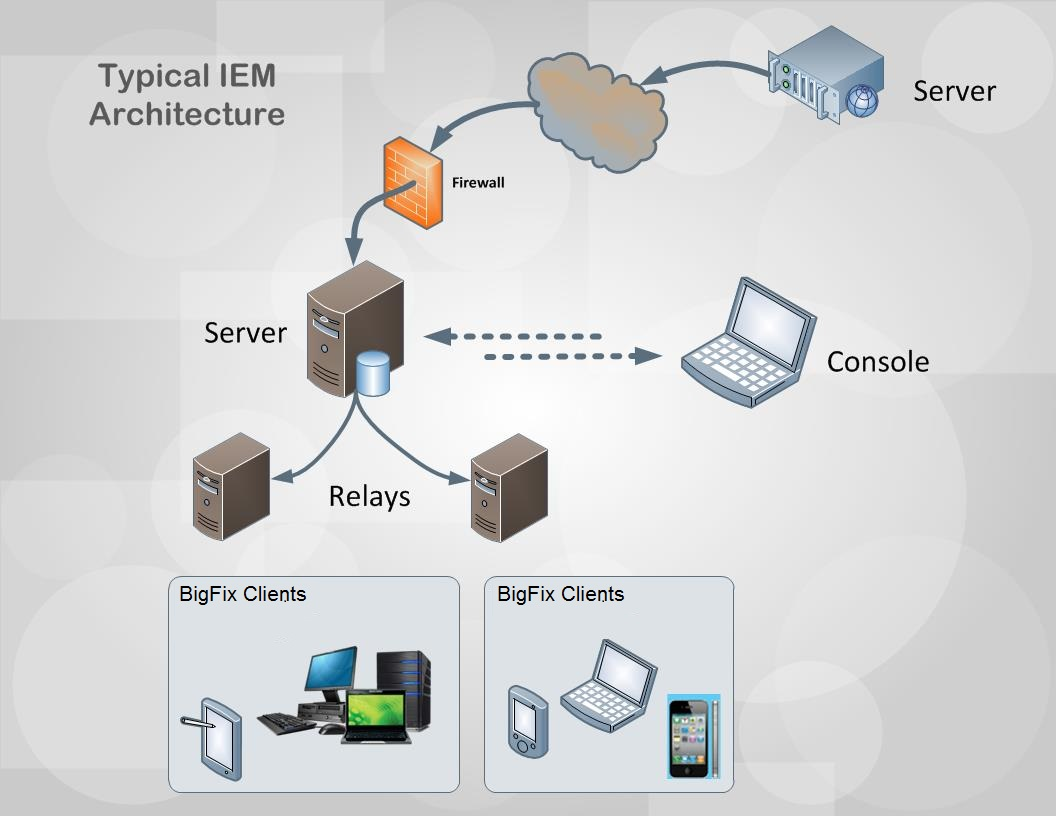
\includegraphics[width=\textwidth,keepaspectratio=true]{capitoli/imgs/IEMArchitecture.png}
	\caption{Un'architettura BigFix di esempio}
\end{figure}
Come possiamo notare, l'elemento fondamentale è il server, il quale ha lo scopo di raccogliere dei particolari messaggi, le Fixlet. Questi messaggi posso essere visualizzati dall'operatore che lavora sulla console e inoltrati quindi, a questo punto ai relay. E' competenza dei relay poi interagire con i singoli client e assicurarsi l'esecuzione delle Fixlet. Le Fixlet, infatti, altro non sono che delle azioni che devono essere necessariamente compiute dai client.

BigFix, da un punto di vista logico, si suddivide in due grandi macro-componenti, la Platform e le Applications. La prima svolge la funzione di layer sulla quale vengono sviluppate tutte le funzionalità dello strato di applications. Questa suddivisione consente una chiara suddivisione delle competenze da parte di progettisti, sviluppatori, tester e assistenti dei clienti. Il team della platform si concentra quindi nel fornire una solida infrastruttura al team delle applications, il quale svilupperà i singoli strumenti al servizio dell'utente.
\subsection{BigFix Platform}
La Platform è una tecnologi amulti-layer che agisce come colonna portante di tutta l'infrastruttura di BigFix. La sua finzione è quella di gestire sia l'intera infrastruttura che i client stessi. I componenti della Platform sono i seguenti.
\paragraph{Servers}
\paragraph{Relays}
\paragraph{Agents}
\paragraph{Web Reports}
\paragraph{Consoles}
\subsection{BigFix Applications}
blablablavlacla isdugfias aiugfiau w aiwegufiue
\subsection{Potenzialità di BigFix}
(wiki IBM BigFix)
\subsection{Fixlets}
(wiki IBM BigFix)
\subsubsection{Il linguaggio Relevance}
(wiki IBM BigFix)


